\section{2015-08-12 Product Manager Interview}

\begin{figure}[h]
\centering
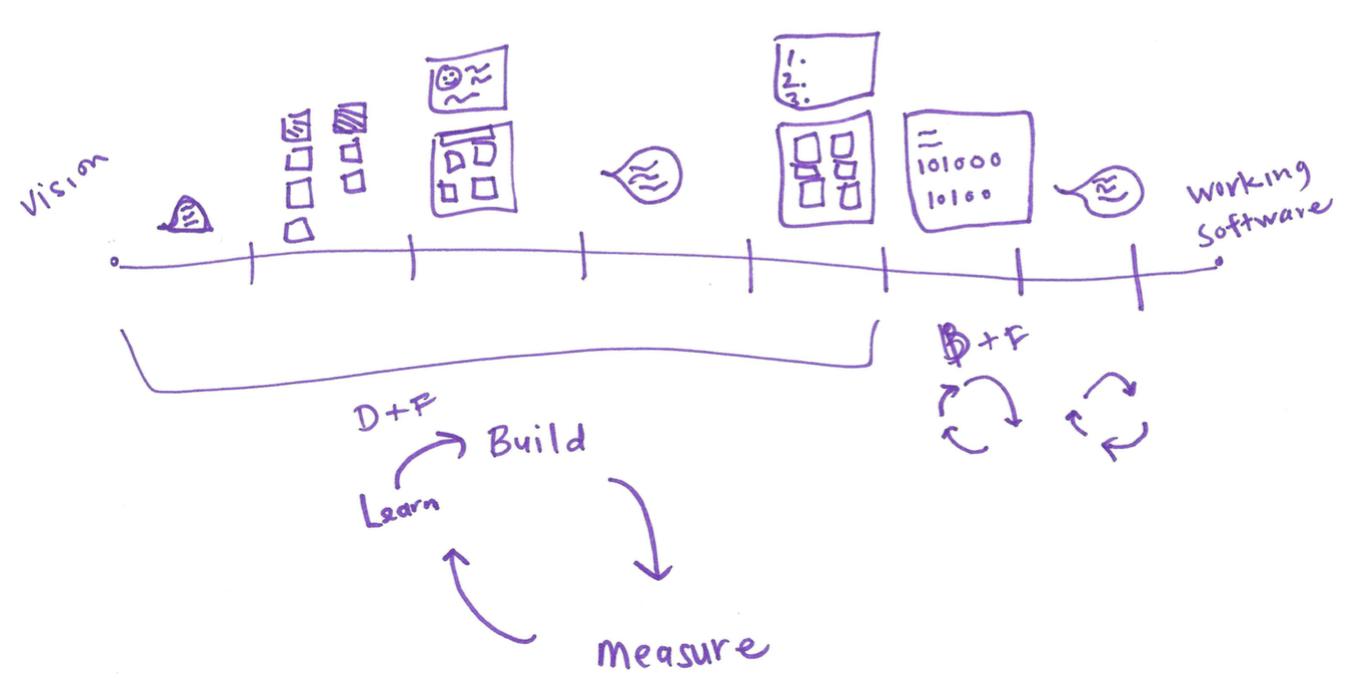
\includegraphics[width=6.5in]{interviews/2015_08_12_pm.png}
\caption{\quotes{2015-08-12 Product Manager's drawing of software development process}}
\label{2015_08_12_pm}
\end{figure}


\textbf{Todd:} If you're open to it, could you, on that sheet of paper, draw out how you view the way we build software? This is completely open-ended. There's no wrong answers. And just take a stab at it.  0:00:21

\textbf{Interviewee:} So I'm drawing a line, it's like product on a continuum. We're gonna have vision here. We're gonna have working. Can you tell I'm a PM coz I'm writing in lines, boxes can't do? 0:00:45

\textbf{Todd:} I love it.  0:00:46

\textbf{Interviewee:} So let's see here. So let's do a couple of lines here. Alright, so let's say, each of these represents two weeks.  So we'll say that the first point, so how we build it at pivotal is that what you asked?  0:01:17

\textbf{Todd:} Yes.  0:01:18

\textbf{Interviewee:} So it starts with having clients.  0:01:20

\textbf{Todd:} How would you build it too?  0:01:21

\textbf{Interviewee:} Yeah, yeah. Totally. The reason I asked about Pivotal is 'cause we're doing consulting. So if you're thinking of product as a continuum, our clients come in in all these different ways of where they the insert. But it starts with a conversation, kind of like a qualifying conversation of like, 'hey, what do you wanna build?', and like 'what's the fidelity of your idea?' And from there, we have a good understanding of if they're at a stage where they can build something, or if they maybe really need to think about it further.  But once we realize ok, they're ready for Pivotal , we'll start with a Discovery and Framing and not every project gets Discovery and Framings, but in the LA office, a lot of them do.  We're trying to get like most projects getting some a semblance of Discovery and Framing.   0:02:04

\textbf{Todd:} When would you not do one?  0:02:07

\textbf{Interviewee:} So we won't do one... I think we can make the case really for all projects could do with a little bit of DNF right? So even if you're like, I know where to build from. So with FYI rather, but for a PM, I'm thinking, okay my role is to help the client understand who are we building for and then what we are building and when? So for the, who are we building for, I think all clients.  It'd be great if we could do some user research with them even if they are like, we did all these user research just to do a quick gut check, like hey this makes sense, that'll be great.   0:02:42

\textbf{Interviewee:} But I think a lot of the times when we don't do them, it tends to be convincing the client or if there's a budget concern.  So they have enough of a fidelity of understanding who their target user is and who the secondary users are and have a persona and are focused on stuff like kinda key factors like, ok, if you're saying you want to build an app for the millennials and for college-age students and for the ages 25-35, that's pretty vague.  We do get that a lot, but we're saying, ‘ok, it's for millennials, so what gender are we going for?' Or is it, ‘what are their behaviors like?'  There's a lot of questions that we can ask on this conversation. and these qualifying calls to say, to kind of fish out, to think if they are ready to work with Pivotal, or if they have enough information for DNF or not. So, does that answer?  I guess that was a very specific answer.  0:03:44

\textbf{Todd:} That was great.  0:03:46

\textbf{Todd:} I interrupted your flow.  0:03:48

\textbf{Interviewee:} No, no, this is fine.  So I'm of the opinion that I would love it if we could have some sort of research with all of our clients and users. Typically when we do a DNF, Discovery and Framing, we do that for 4 weeks on average, sometimes it's up to 6 weeks depending on how many users they have and how many people they want us to focus on.  But we typically really try to work on 2 to 3 target users being 1 primary user and maybe 2 users of the system that kind of insert in their day.  And then we've done a 2 week of design first or Discovery and Framing but really it's just 'let's talk to some users and validate some ideas.' But the whole goal of this Discovery and Framing process is to do a couple of weeks of talking to users, of about 2 weeks and that's when we're doing some of those exploratory interviews, kinda turn it into elicit narratives to understand what their behaviors and what their days are like.   0:04:51

\textbf{Interviewee:} And then from there, we can isolate what are some of their pain points and what are some of the frictions and inefficiencies and how are they capturing data and what are the tools that they use and who are the people they're talking to.  From there, I guess one thing I didn't mention which is important is to say, what are the product goals that our clients have?  And what are some of the assumptions that they have about their products?  About their users where their products can help solve their needs.  We go into these user research thing like, alright, here are some assumptions, hypothesis that we have, let's test them. Out of that output of user research is that we have this, we do some synthesis and analysis of all of the things they're talking about.  We record the things that we saw, so if they're in a cubicle and they have tons of printed out papers because what they do is they get stuff by mail and then they have to scan it in.  Those are the things that we're seeing that are part of their day that can affect them.   0:05:54

\textbf{Interviewee:} What did we hear, like things that they're telling us about their day, and things like we felt that they're telling us. But maybe there are some subtext and some nuance there saying everything's great but their faces are really strained and you can tell they're really frustrated and their posture has changed when they're talking about certain subjects. Kind of taking all of the things that recording from our user sessions and then coding it by what we saw, what we heard, what we felt and then finding themes. What are users talking about? Usually when we do research, we try to do 3 to 5 users, so that way we have a good cross-sample and in case there's any extreme people that we meet, it kind of helps us give a better analysis, better data sample. So we'll kind of call all the information that we have and we'll go to them, too.  So we'll go to their cubicles or wherever their workspaces are. So we want to get a sense of their environment. Cause there's so much contextual information there that you can't get just from having a phone call with someone.  0:07:02

\textbf{Todd:} Yes.  0:07:03

\textbf{Interviewee:} So, then, that's usually about a couple of weeks doing some researching.  As we're doing the researching, we're capturing all of our information on notepads and then we're doing what we call infinity mapping, affinity mapping.  We'll get one of those big phone cork white boards and we'll take a listen to the recordings of when we're doing user research or if we can't record just looking at our notes ‘coz our notes are like, you're almost writing verbatim what people are saying.  Coz you don't want to put all your analysis in there at this point, you just want to get them to talk and get it all in, and then we'll take each kind of idea and we'll put it on a post-it note and we'll have a bunch of post-it notes around and they'll be coded by what we saw, what we heard, what we felt, and then we'll start seeing themes around this post-it notes.   0:07:54

\textbf{Interviewee:} So there's this one user that said there is a lot of things around education and tools and timeline and whatever it is.  Then we started noticing trends, so we'll start taking those nuggets and we put them across this themes and then we'll do that to all our users; and then from there, we'll do another round of synthesis and the ideas are going to keep condensing.  So then we have a synthesis of all the people we talk to and what the overlaps are and the themes of what their day is like, and the behaviors they drawn during that day.  And then after that, we'll map out their day, like what are the tasks that they're doing, and then map out from the tasks all those insights rather not insights but nuggets of what we heard from them, that we kind of collectively called down and condensed and we'll put those against the tasks.    0:08:43

\textbf{Interviewee:} So when they need to schedule a user for an event, these are all the things they said about it, or these are the things we saw and the things that we felt.  So then what's cool about that is we do that for every target user and you can map them out.  So you say 'here are three target users, here are their days and here are all the intersections of their days'.   So you can tell visually, 'oh, you know what, when this person does something, you notice the next thing, like, these two people are affected.' And then you can start isolating pain points and inefficiencies and you get these really nice overlay of what the system, not the digital system but just the users in the workplace and what their days look like.  So when I'm mapping out the process, I'm thinking of conversations, that's a little talk bubble.  0:09:43

\textbf{Todd:} Ok, I like it.  0:09:44

\textbf{Interviewee:} And then I'm having doing some synthesis. Someone do a little post-it map.  0:09:51

\textbf{Todd:} Ooh, I see the post-its.  0:09:53

\textbf{Interviewee:} There you go.  And then from that, we say, 'ok, based on our research, this is what we say a persona or what this user looks like.'  We think of 'what do they need? What are the tasks in their day and what do we need.'  So we pull out insights from that. Like, this user really has trouble communicating with the other people on this team because they don't have the right communication tools setup or whatever that is. They need a better communication system.  Once we have these needs, and bits and insights of who they are and what they need, then we can say, "all right, how can our products solve these needs?" So then we say, 'we have some product ideas based on what their needs are, let's validate them.'   0:10:55

\textbf{Interviewee:} Then we'll go back and talk to the users. We'll drop some wireframes and say, "all right, based on what you guys had said, we feel that here's a quick prototype, clickable prototype" And we'll use invision.  We'll say, "Why don't you click around? What do you think about these things?" we'll do some user testing there.  And then from that information, we'll further validate or dis-validate our product ideas and we'll do another product evolution but kind of the output of this 4 week on average DNF cycle as that you'll have Wireframes and then you'll have some personas. You'll know who your end user is.  You'll have empathy drawn for your end user which is the whole goal. You'll have a problem that's been framed and validated.   0:11:38

\textbf{Interviewee:} So that way, it really de-risks development cause it's pretty great to come in to development and we know that when we're making product decisions, we can go back to this research.  We're like, "oh, if we're going to do this or this, like, what do they actually need? Like what was that they talked about that really indicated this is the right approach?" It also helps us speak a language that our users speak.  Which is really important for the development team but all the other stakeholders involved in the process.  0:12:05

\textbf{Interviewee:} Words are everything, right? So we want people to be kind of on the same communication levels of talking how their users would talk, so that way it helps us draw all that empathy throughout the entire development process coz you still need to draw on that, you know 6 weeks, 3 months, however long into the development cycle until you're releasing. Right to be able to have that insight of what they want. I think the cycle is... Let's just say that you've done some analysis and you've done some wireframing, and then after that, we'll talk to users again.  After that, we'll do another set of wireframes. We'll also do some persona mapping here as well as making these wireframes.  And then after we do that, we will create a feature list.  0:13:13

\textbf{Todd:} Yes.  0:13:14

\textbf{Interviewee:} So, we'll say, like, we're not gonna…  Like, what could the next you know 2 to 3 kind of epic areas. We'll say, let's give some insights here.  Like, maybe, we have 3 insights and 3 needs.  Let's do 3 feature ideas and how do these feature ideas map these needs?  So we write these feature ideas and we'll say, down in the documents and user needs this and we'll help them achieve their goals.  Business needs this and this will help them achieve their goals.  We're always aligning user business needs throughout the entire process. So then when we get into development, we'll just make a little terminal, I wish I had multiple colors.  0:14:00

\textbf{Todd:} Next time, you'll have to bring your can.  0:14:03

\textbf{Interviewee:} So, when you're getting into the computer, when you're getting into development, you're able to have a backlog that's been built.  You have the first couple of weeks of features.   0:14:17

\textbf{Todd:} Yes.  0:14:18

\textbf{Interviewee:} You have some ideas and you start building and then once you release something, which could be in a week or could be a couple of weeks depending on what you're doing.  But once you get into the first bit of business value working software, then you can go and you could talk to your users again and then you learn from them and then you continue on.  So at that point, what you're doing is you're building something and then you're measuring it.    0:14:45

\textbf{Todd:} Yes.   0:14:46

\textbf{Interviewee:} And then you're learning from it right?   0:14:48

\textbf{Todd:} Uh-huh. Yes.  0:14:50

\textbf{Interviewee:} And then you're going back to building, right? So that's what we're doing for this whole process. So the feedback loop is really important.  I think, when I'm thinking about the extent, like the depth of all these research, you don't need to have a DNF to do any of these research, right?  You don't have to sell that in, you can do...  So the training that our designers and our PMs have, and now we're trying to have our developers be exposed to it, as well.  To say, ‘ok, developer, you get a client project. Development starts tomorrow, you can still talk to some users.  You can still setup user testing.'  And you can do that throughout the entire process.  So it's almost like this whole upfront part, with like the DNF.  You're making little DNFs through it, right?  So whoops, it's really you're taking this and you're kind of doing like DNF cycle.   0:15:42

\textbf{Todd:} Yeah.   0:15:43

\textbf{Interviewee:} Whoops, and you're doing that here, and then you're going to do it again. So, like each week, you might be bi-weekly.   And that is ideal, right?  But sometimes you don't get the users?  So there's a lot of, kind of…  You have to be pretty scrappy with how you do this sometimes, you don't just get this nice set of users at your disposal, you know; but it's so important and I think that's something we do a good job with is convincing our clients, like, we wanna de-risk this for you so this is how we can do it.  I mean go, it makes sense.  It's very practical stuff.  It's not rocket science honestly.   0:16:20

\textbf{Todd:} Now are you currently PMing a project?   0:16:24

\textbf{Interviewee:} I am.   0:16:25

\textbf{Todd:} I kinda noticed that every project, like, by its grain, is different.  I mean there's some commonalities but each one has its own, it's like children, each one has their own personalities   0:16:33

\textbf{Interviewee:} Oh, my gosh, yeah totally.   0:16:35

\textbf{Todd:} So, your current project, when you think of its uniqueness, what are the challenges or pain points that make this particular engagement interesting?   0:16:47

\textbf{Interviewee:} Sure, you know I think that, I think this is truly an opportunity and cool but it's a huge challenge.  We're working on a recommendations engine, and this recommendation engine, what does that even mean?  It's like pretty broad language and so we are, and you know, the term algorithm gets thrown around a lot.  It's like, what does algorithm mean.  And we also have some data scientist in the office, so when we talk about algorithms to them versus our clients, different connotations of the word.   0:17:21

\textbf{Todd:} They talk about the heuristics as well?   0:17:22

\textbf{Interviewee:} Yeah, they do actually, that would be more when we're talking to our data scientist coz our clients aren't quite to that level of knowledge.  But I think that's one of the challenges is making sure, you know, as PMs, that we're helping them deliver value, and they're not getting overly complex before they need to.  They say, they came to pivotal because they want to build this recommendations engine.  We're like "cool, but before you build this recommendations engine, you need an application that has a certain amount of data and functionality before you could recommend anything, you need people, you need conditions, you need affinities, you need restrictions,” or whatever it is.   0:18:05

\textbf{Interviewee:} So it's been our process to get them to, you know, and they've been really supportive of it, but they excited right?  So it's like managing their expectations throughout this whole process to be like, "don't worry we'll get to it, but we need to get to all these other things."  And what we get to, maybe, a little different than what you expect and maybe we don't get to it all, right?  So we're actually at the end of the engagement and we're trying some really cool things that are little less sophisticated than they expect but fully meets their needs plus more.  So I think that one of the challenges with this project is for them to say, "Hey, ultimately, does your end user, are they able to do the thing that they need using this recommendations?  And do these recommendations make sense to them?”  So, yes, cool, that's success to me.  They can schedule, so it's a scheduling app and then, and the goal is really to schedule these users to events.   0:19:04

\textbf{Todd:} Yes.   0:19:05

\textbf{Interviewee:} And then this recommendation engine to make it easier for the scheduler so they don't have to think about why they're scheduling people but they're like "oh, well i can schedule quickly coz I don't have all the burden of detail of why this person can go here and this person can't".  Coz it's very intensive type of scheduling that they're doing, that's all based on this…   0:19:24

\textbf{Todd:} A lot of constraints?   0:19:25

\textbf{Interviewee:} Yeah, well you know I won't even say it's a lot of constraints actually coz I think that actually one of the challenges is that I feel like we almost like spending a lot of time on the edge case right now, that the bulk of the app that don't necessarily need this.  There's a little bit of proximity and some stuff that makes it easier. So I would say that recommendations engine I say in air quotes like 101.  We hit and they can do pretty early on in this application but we some of the other stuff they're… they have, they just manually take this historical information that the schedulers has and just adapt it into the system or at the system; but then they also need to see how the schedulers use it before adding more complexities, right?  Because I think they have data in the system that they can add to this recommendations engine but we don't know if that is really what they need. We don't know what's the right data that they're looking for this?  So I think they want to put a lot of work into something they are not ready for, but we strike that balance.  0:20:29

\textbf{Todd:} So given the challenges and the uniqueness of this project, have you found yourself tethering or adjusting the way we work to achieve those goals?  0:20:42

\textbf{Interviewee:} I think that.  So, like, agile it's like a set of different tools, right? So I don't think there's one way to do any of the things that we're doing.  I think there's a baseline of process that we certainly need to adhere to.  Like we always have a planning meeting, we always have a retrospective, we always have a stand-up.  I think that's helpful for the communications side coz most problems are people problem, so it's nice to have a good strong communication system in terms of like tools that we use to do, to make product decisions, to develop wireframes.  0:21:20

\textbf{Todd:} Trying to do a...  Like you do have a baseline that we all use.  I'm trying to find the, what are the little recipes that you pull off to spice up the soup we're making.   0:21:32

\textbf{Interviewee:} Yeah, I'm sorry i already forgot what specifically you asked for that question?   0:21:37

\textbf{Todd:} Oh, I guess this is pretty open-ended but curious like as a PM, do you have these tools that you just like almost like playbook items that you could go and reach for?  I'm kind of curious in the particular project which things were you reaching for than maybe having reached for in other engagements.   0:21:56

\textbf{Interviewee:} Right, right.  I think for this one, so this one I actually came in toward the end of the engagement coz I was in a different project and I'm not fully working on this project.  So I have a couple of things I was billed for which is a very unique thing at Labs that doesn't typically happen. So I've been doing much more like enablement teaching on like how I make product decisions, how I cut down on really thick backlog.  I think for we're using data science, so that's something unique for this engagement.  We've been pairing with other data scientists and I've been doing a little more like kind of high level conversations, like really our engineers are working with data scientists.  But I haven't really done anything I think that's been super kind of unique that I wouldn't do in another project.   0:22:55

\textbf{Interviewee:} The recommendation stuff is different, I haven't worked on a project with recommendation stuff, so there is been a bit more like a designer who has worked on those projects a while ago set up this really nice like set of equations that have to do with decayed log and some other kind of basic loose algorithm need, just some equations for waiting.  So there's been some additional research I've done on recommendations and, like, kind of spending a little bit more time with the developers thinking through how we would do certain weighing and sorting but I wouldn't say that there's anything that has been so unique to this project that I haven't applied to another project.   0:23:34

\textbf{Todd:} When you described enablement teaching a moment ago, is that for the client's PM or who are you enabling?   0:23:41

\textbf{Interviewee:} Oh, the clients.  So the founder, the CEO is our PM for this project.  So I've been working with him just making sure that there's the basics of, this is how you build a story.  Like using that mnemonic of invest rate, like, it's the right size and the right value and have the right description and then there's, you know, kind of, worthy end of the engagement right now.  So you wanna do all these things and you think critical for your MVP and for going live is this, this and this. How can we think about search instead of having this isn't specific for this.  But an idea would be, like, instead of the doing a search function, which can be, like, take all the time that you give it, maybe to control F on the keyboard and then you can see, you could search that way.   So kind of trying to figure out some like ways where he can still get the value he needs, where he doesn't need to add so much complexity to it, you know.  Like he wants to do this kind of write up kind of HR function. I'm like, "well you have email right now", I'm kind of like, "how many write-ups doing per day?", like "can you capture this on Google drive spreadsheets right now and track the write ups for these people that way instead of putting in these functionality", you know,  0:24:58

\textbf{Todd:} Into the tool, right?   0:24:59

\textbf{Interviewee:} Into the tool.   0:25:00

\textbf{Todd:} Yeah, it's interesting coz the idea doesn't... I've worked with the founder on the recommendations engine with some graduate students and it's just interesting how I picture he had some…  He kind of want to think things will work in a certain way and wasn't always clear, like, if his solution would solve his problems.  And so I feel, like, as a pm, I kind of wondering if you were sort of massaging, make him to, like, re-think his solutions and then understand his problems first?   0:25:29

\textbf{Interviewee:} Every day.   0:25:30

\textbf{Todd:} Ok.   0:25:31

\textbf{Interviewee:} Oh, every conversation.   0:25:32

\textbf{Todd:} And how does that work and do you like facilitate that?   0:25:34

\textbf{Interviewee:} Well, I think a lot of it is I think about, like, ok, again this kind of goes back to like what are your business goals.  Like, you have a lot of business goals but what are your top 3 business goals? Who are your top 3 users and what are their needs?  So when you're making decisions and if it doesn't align with these, or if it kind of align with this, it's really easy to be like, well, this is your budget, this is how many hours you have left, what's more important?  Ultimately there are other ways of thinking about it. So there's a lot of, use some facilitation techniques like, I'm sure you've heard of like a Dump \& Sort or 2x2, right?   0:26:15

\textbf{Todd:}  Oh, 2x2 yup.   0:26:16

\textbf{Interviewee:} Yup. Yup. So there's things that, like, what you'll do when it really comes to \quotes{I wanna do everything.}  So there's a point in this project not so long ago where the development team didn't see eye to eye on this path because this path for now we kind of getting into the heavier recommendations stuff.  And there's a lot of opinions on how this should be done.  So we did a workshop where we did a couple of rounds of Dump \& Sort and 2x2s, so how we did it was there was purposely a break in between with lunch.  The idea was like alright the question I asked was, "what do you think the path is for what we're trying to achieve" or something like that.  It was more specific it was like, "what do you think we should be doing?", like, let's do a Dump \& Sort on that and so everyone did it and we have variety of ideas and we then we put it on a 2x2 on complexity and value I think, value on development of complexity in value.  0:27:17

\textbf{Interviewee:} So coz we're thinking like time, and then like impact. So we did that and we got everyone closer to the same page at the end of like everyone did agree that this is the first thing that we should be working on now and this is the second thing.  And then we said, \quotes{ok, cool,} knowing all that, what are some of the technical implementation details coming from that.  So we did Dump & Sort and that we prioritized again.  We didn't do a 2x2 at that point.  We just kind of prioritized some ideas, then we had lunch, we came back and I asked the same first question of, so what do you think this same path forward was?  0:27:51

\textbf{Interviewee:} And it was interesting because my hypothesis is that they'd be more aligned but they weren't. They actually were, they were closer but what happened was after we did that, it was just the Dump \& Sort, we didn't do another 2x2, but then we said, \quotes{ok, so what are, let's talk about this.} What came out of it really quickly, because we already framed all these conversation was this idea was like, "oh, what if we do it this way?', and someone was like, "oh, that's great." so everyone had consensus within maybe 15 minutes after we had this like round 2 of asking the same question, people looking like they were kind of divided.  I think it was because people felt heard that there is another opportunity to talk through some of their thinking, that they were more amenable to other ideas and we're able to get to that open creative space.  It was really cool, but I was not expecting that we'd come back and everyone would be like so diverse again in their thinking.  It's interesting, so I guess that was different.   0:28:51

\textbf{Todd:} What would you do with the client that refuses to prioritize?  They would refuse if you brought them down to the table and say, \quotes{let's do a Dump \& Sort}, and they say, \quotes{No, we won't do that. Everything is of equal priority.}   0:29:04

\textbf{Interviewee:} Oh, so I've done that a lot and I've never had someone say no.  I don't know.  We just keep working on it in different ways.  So I think like...   0:29:14

\textbf{Todd:} It all has to be done by this date.   0:29:16

\textbf{Interviewee:} You know the date-time too, that's definitely come up, but I've never had someone who's been that absolutely no, like, I won't play because there here to work with us and I think they understand they're spending quite a bit of money working with us; even the ones who might not have that true number in their head, they get that sense of "I'm here to make something work". I think that people come in here for the most part, I haven't witnessed people that have been so 'I'm closed off, I don't wanna do this'.  But again it's kind of contextual, so it's easy for me to create like scenarios or ideas once I know what the product is.  So I'll tend to say, ok, because there's a lot of, like, writer's block or prioritization block.  Part of our goal is to be facilitators and to pull out ideas and say, like, "ok, cool.  You want these 4 things to be done by this timeline, so let's just, lets' focus on one.  What do you think the number 1 is, let's start somewhere”.  And them like, "it's all equal”, but we'll say this", and then we're like, "ok, next one, is this one more important or less important than that one?", "Oh, it's just as important", and then alright, so let's dig into to it.  \quotes{So what makes this more important?  How does it achieve?} I might start writing "what are the goals of the product here?" and then "who are your users?" and then I can even say ok.  And then I'll prioritize that.  Like, some will have some ideas and stuff like "here's all the things that's important and we'll try to do some prioritization of product goals. We can usually get somewhere when we prioritize something and then I can match whatever it is that we're talking about against that.   0:30:57

\textbf{Todd:} Yeah.   0:30:58

\textbf{Interviewee:} It's, like, how does this help you get to your timeline faster, right? How does this get someone to do this easier?  Ok, cool, so is this to be more complex than that, so then maybe timeline's the big thing here.  Then let's go with the thing that seems least complex.  There's a lot of that, like, we're kind of totally use that, like, you know, time-quality-budget triangle, the project manager triangle you always hear about.   0:31:25

\textbf{Interviewee:} So there's a little bit of that, but we have fun with it, too.  Like I try to, you know, people come in here with so many different reasons and perspectives on what they're doing and why they're here and so I try to keep it as light as possible, too and try to really decouple the emotions and the behaviors and kind of lean on the process more.  So it's not, \quotes{oh, your guys}  fault that you're not agreeing.  It's the process, we need to be able to facilitate an environment where we can talk about our ideas and prioritize them together, right?  So we really try to lean on these consulting tools and process these and whatnot to make it a little bit easier for people to get their minds out.  And the Dump \& Sorts nice because it's a really cheap and easy way of getting people just to get their ideas out and in the beginning they might have nothing or they might have the first three ideas really fast and like oh now i have nothing. and so they will say, great whatever you want, like, maybe an earthquake can shut down your business or you know whatever the prompt is, like, we'll think of some absurd things.  Write bananas if you need to or whatever.  You know what I mean?   0:32:41

\textbf{Todd:} From your perspective what is the purpose, what is your goal of the IPM?   0:32:47

\textbf{Interviewee:} Oh, so I think the goal of the IPM is to say, \quotes{Alright, where have we been and where are we going?} So this last week, I always start with the… I guess it's about getting people on the same page and with understanding the same vision and understanding what the goals are of the product for the week ahead.  I think it's important to say "alright, here are the big things, here's how our environment has changed based on what we've deployed and you know here's currently what's being worked on today since waiting for this meeting.  Are there any questions about it?  Is there anything that we need to know that's being worked on now that might change these future stories?" and then we go into each individual story and we say, "Alright, here's our treasure map. Let's talk about some of the hidden complexity from this."  It's not about, in my perspective, to have developers write out every single tasks and implementation details but it's kind of that space to have enough of a conversations so that you can estimate complexity as a team for a specific feature story, and that you can leave that meeting having a good understanding of \quotes{hey, here's how the next two weeks look like knowing that things change.}   0:34:09

\textbf{Todd:} Nice.  So you spend some time at the beginning of the IPM reviewing what happened recently. And it's like that 5, 10 minutes?   0:34:19

\textbf{Interviewee:} Yeah, well, so let's say the IPM submit in like an hour, so the first I might say, like, "hey, I'll have tracker up."  And I'll say, "here are the largest things that we delivered last week, just as you're thinking about complexity, here are some of the things that you might we learned that this integration point is behaves differently than we thought, and we have some research that we need to do."  But it's like a minute to a couple of minutes, we don't spend a lot of time, it's like a very quick recap.   0:35:00

\textbf{Todd:} Yes.   0:35:01

\textbf{Interviewee:} And then we'll say, "Alright.  Here's a couple more minutes and let's talk about what we're doing right now.  So is there any question on the stories that you're working on? So here are the stories that are in flight."  The planning meeting tends to be Mondays so there's, you know, depending on your team size, but if you have 2 to 3 pairs or 1 to 3 pairs, there's only a couple of stories that are being start or that are started.   0:35:22

\textbf{Todd:} That's true. Right.   0:35:23

\textbf{Interviewee:} And we don't go through like, all 6 stories from last week or whatever. It's just kind of quick context coz it's Monday and people have a weekend, just want to remember what we're all working on.  But then my agenda as a PM is I want to have all the stories pointed with complexity and that there's conversations had to enough fidelity where people have an understanding of what's going on and that they also know who to ask.  And if there's any blockers or dependencies that I need to know about so I can start unblocking things.  So if you think about it, if you're doing, like, what is it, 2 weeks, 1 try to go over 2 weeks of work so the current iteration, the next and if you have (this is for non-engineers) say 10 stories, right?  So you're trying to get through a 10 stories in a week, that's pretty high but whatever.  And so have 20 stories that you need to get through, and you want to spend a couple of minutes on each story.  Let's say you do 3 minutes on each story, so that's a full hour.  It's all about saying that pre-IPM or just like, not even if you're having a pre-IPM but all that you need to so much research and like good work and write the right stories and that goes as soon as possible.   0:36:36

\textbf{Todd:} There's a lot of people in the room.   0:36:37

\textbf{Interviewee:} Yeah, there is a lot of people in the room.  So it's about finding your rhythm but I think the goal is to make sure that you have a brief overview and that you can tell if it's taking longer than that few minutes per story.  The story's not ready and you immediately got to pull it in and put it in the Icebox.  That's on the PM to really be true to themselves and make sure they have that the ability, it's part of their facilitation to be like, ok, I think there need to be discussion so let's pull it out.   0:37:06

\textbf{Todd:} Yes, interesting. I was on a project where I've realized that we didn't really have iterations.   0:37:15

\textbf{Interviewee:} Oh, interesting.   0:37:16

\textbf{Todd:} We were actually very present with the work, we would just show up and do whatever's next on the backlog and the purpose of the IPM was basically to make sure there's a pointed the stories in the backlog.  And then it was really interesting moment for me.  Coz there's other agile techniques where you actually agree upon what you're going to do with your iteration like scrum.   0:37:40

\textbf{Interviewee:} Yup.  Yeah sure.   0:37:41

\textbf{Todd:} Kent Beck's Extreme Programming actually says you should do that, that you should actually commit to the work you are doing that week and I find that at least the projects I've been on were much more present that if a PM in the middle of the week says we have to change what we're doing, we just do that.  We alter what we're doing, we're very flexible and so for us on my teams, it doesn't really matter what day of the week we do the IPM on.  Sometimes, we do that on a Wednesday.  It's just that when the client is available, it really tends not to matter. It's just interesting.   0:38:17

\textbf{Interviewee:} I agree with that.  Like, I don't think we have this kind of Monday, like start of the week with the IPM, Friday retro but let's say you're working on 1 week iterations and your releases on Tuesdays, then when does your week start then.  Maybe you have your retros on Monday and you do your IPM on a Wednesday or something like that, Tuesdays your retros, however.  I think the goal is to be flexible as you're saying. You know, I think, it's all about your team rhythm and what you guys agree upon as this is the process that works well for you.  So I do think it's nice to have this kind of like you know, XP or your agile, whatever your kind of flavor of process that you're using and then you can adapt to it wherever you need.  You know I think 1 thing we need to watch out for consulting is our clients have different levels of backgrounds in this work.  And so we want to teach them like a good base level process so that they could then figure out kind of what their version of it is, and then also, the kind of speaking to them, no idea of an iteration.   0:39:27

\textbf{Interviewee:} I'm on board with that but you don't want it to be too jarring for people so when you're pulling stories in and out of the backlog too much within a week, you just want to make sure you're not doing too much context switching and that you're not, that work you're doing or whatever planning meeting that you're doing, it's noted and that you're kind of bringing that into your week. I don't know, I'm with you; I think it's great when you would need to be flexible, I would like that, I would actually prefer that. I just worry about the clients and their ability to work in those kinds of such flexible environments you know.  I do like that we give them this kind of, for their first engagement, we also have clients that come back for lots of different engagements, I don't know. I like it, I think and I've had teams where we've just been able to move things in and out but it's also been that the developers feel like there's not much thrashing and they're ok with it. I think it's easier for PM to do that but harder for an engineer to do that.  I think there's so much more thought going into the tables that they're working on into how they're structuring the project. I think it can be done in the right way but I'm always really conscious of that.   0:40:43

\textbf{Todd:} I think the saving grace is engineers don't want to work on non-pointed of stories so there is a gating factor. i mean, if i just dropped in 10 stories at the top of the backlog and they're not pointed, someone in the team's gonna say "hey, wait a minute, we need an IPM."   0:41:01

\textbf{Interviewee:} Well, I think it's scaled to, right?  Like a couple stories versus 10 stories that's different thing but...   0:41:08

\textbf{Todd:} It's like if I'm turning a steering ship a lot, there's gonna be push back and say, "wait a minute, we need to talk about this stuff."  I'm just not gonna pick up, and if I slip one in then you know that's ok.   0:41:20

\textbf{Interviewee:} I think it's like what's reasonable for your group, too. Like if you're finding that you can develop deliver value and you're testing with user and you're not doing so much big change that like...  I think you'll have to have healthy user testing process if you're gonna do big change really quickly as well.  Coz if you do all these change and then you never check with users frequently, then how well do you know that the change you're doing is right? Coz you can build in all these different directions and I'm all about like I do side on small experiments that you're testing, so when you're doing really big experiments or just more risks with what you're doing.   So I guess that's more of in terms of the pointing, you can have developers point, you don't have to be in an IPM to point, I guess.  I think that's a misconception like you can have a developer pick up a story and point together or point with 2 pairs if you want that kind of...  But it also depends on what you're working on, on what you're pointing, like a text change versus like an integration addition.  Those are very different conversations, too; so I think it is really contextual. That's what I would say.  But the trashing is what I'm always worried about.   0:42:34

\textbf{Todd:} Yeah, yeah.  That'd not be good.  Thank you.  You've been very delightful.  I think we could go on forever but I think I can't. So thank you so much.   0:42:45
